%%%%%%%%%%%%%%%%%%%%%%%%%%%%%
%%% - Team Organization - %%%
%%%%%%%%%%%%%%%%%%%%%%%%%%%%%
\subsection{Team Organization}
\label{ssec:TeamOrganization}

%Team Organization Chart:
\begin{wrapfigure}[8]{R}{0in}
	\centering
	\raisebox{0pt}[\dimexpr\height-2.5\baselineskip\relax]{
		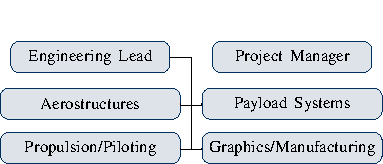
\includegraphics[]{team_organization_chart.pdf}}
	\caption{BYU DBF Team Leadership Organization}
	\label{fig:personnelassignments}
\end{wrapfigure}

%Introduction
\Cref{fig:personnelassignments} depicts the overall organization of our team structure, with arrows indicating who defers to whom. 
Note that the engineering and project management structures are treated separately as indicated by the blue (engineering) and red (management) arrows in \cref{fig:personnelassignments}. 
Each of the listed subteams is comprised of a lead and members.
On the engineering side, design and process decisions requiring single subteams are made by the respective team leads in council with their subteam members.
Multi-disciplinary decisions are made under the direction of the Engineering Lead in council with the subteam leads.
Although the management structure allows the engineering side free reign, budget decisions require approval from the Project Manager, and all leads are accountable to the Project Manager for their respective deliverables, including portions of this proposal and the final design report.
A breakdown of the specific duties and required skills of our subteam and leadership members are described in the sub-subsections below.

\subsubsection{Engineering Lead} The Engineering Lead has good decision making and leadership skills, qualities the BYU Aeronautics Club seeks to develop in all of its members. 
The Engineering Lead operates as a systems engineer and has a well rounded understanding of the various subsystems and both design and testing experience.
\subsubsection{Project Manager} The Project Manager acts as a logistical overseer for the team, overseeing \textit{all} the team leads (see the red arrows in \cref{fig:personnelassignments}) on the various non-engineering tasks that need to be completed. The Project Manager has excellent organizational and technical writing skills, heading up proposal/report writing, budgeting, and scheduling.
\subsubsection{Aerostructures} The Aerostructures subteam members are responsible for the airframe design and testing. They have expertise in aerodynamic and structural analysis and testing, including design skills in hand calculations and computational analysis tools. They also have experience with wind tunnel, glide, and structural testing methods.
\subsubsection{Propulsion/Piloting} The Propulsion/Piloting subteam focuses on designing and testing the propulsion system efficacy and efficiency. Members also have skills in electronics related to the propulsion system as well as piloting skills used in simulation and flight testing.
\subsubsection{Payload Systems} The Payload Systems subteam is comprised of members with multi-disciplinary skills in structures, manufacture, design, and mechatronics. They bring these skills together to brainstorm, prototype, and test various payload system solutions.
\subsubsection{Graphics/Manufacturing} The Graphics/Manufacturing subteam has skills in CAD design as well as graphical marketing for the team. They also assist in the manufacturing of prototypes and testing apparatus, as well as oversee the construction of the final, full, aircraft.